\chapter{\label{sec:prior-art}Existing Solutions}

The idea of making it easier to interact with low level hardware from a \gls{PC} is not new. Several solutions to this problem have been developed, each with its own advantages and drawbacks. Some examples will be presented in this chapter.

\section{Raspberry Pi}

\begin{figure}[H]
	\centering
	\begin{subfigure}{.5\textwidth}
		\centering
		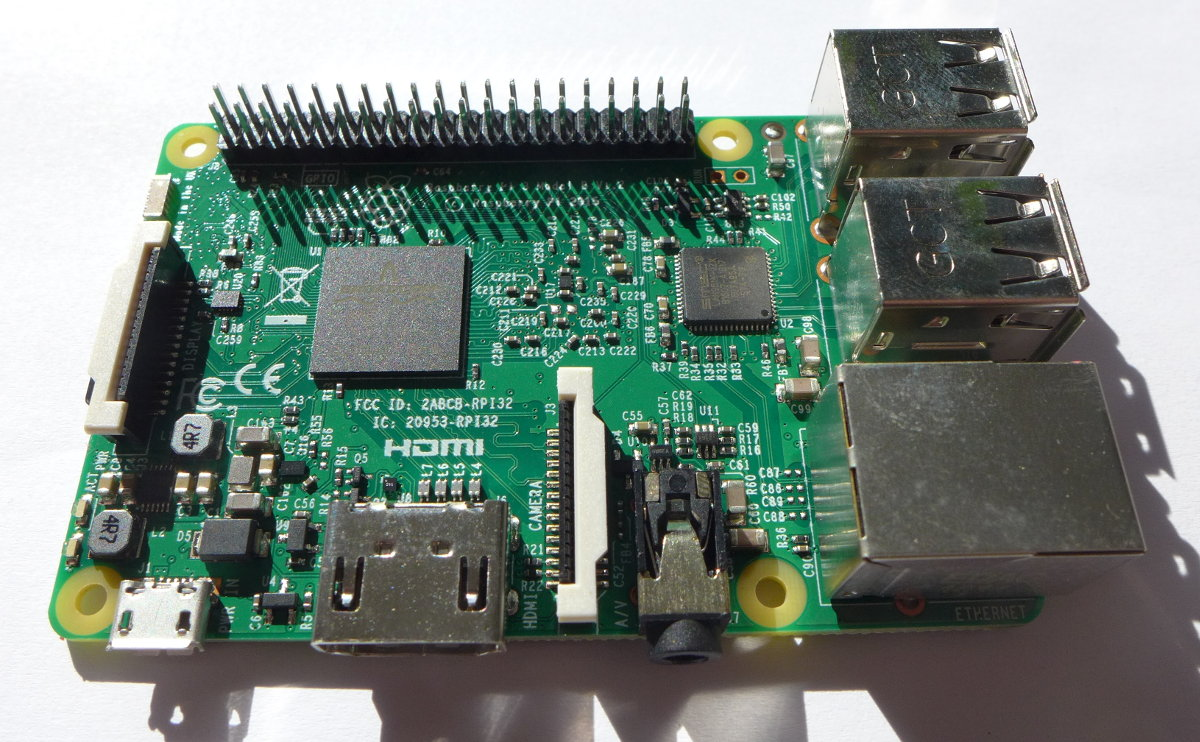
\includegraphics[width=.95\textwidth] {img/pi3-photo.jpg}
		\caption{Raspberry Pi 3 Model B}
	\end{subfigure}%
	\begin{subfigure}{.5\textwidth}
		\centering
		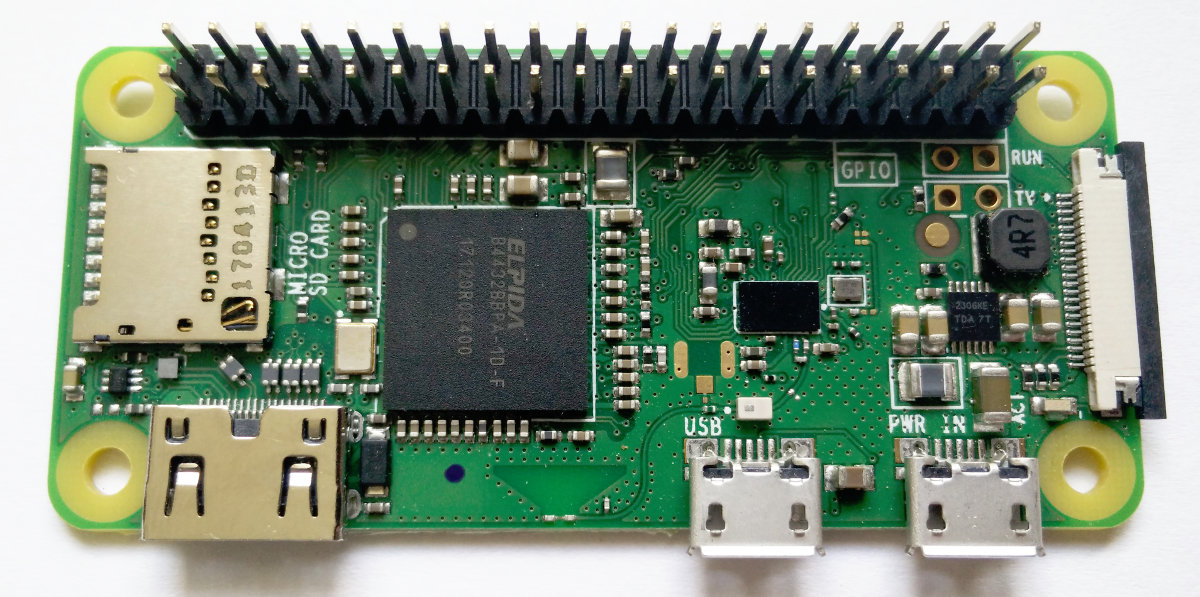
\includegraphics[width=.95\textwidth] {img/pi0.jpg}
		\caption{Raspberry Pi Zero W}
	\end{subfigure}
	\caption{\label{fig:rpi}Raspberry Pi minicomputers}
\end{figure}

The Raspberry Pi's \gls{GPIO} header, a row of pins which can be directly controlled by user applications running on the minicomputer, was one of the inspirations behind GEX. It can be controlled using C and Python (among others) and offers \gls{GPIO}, \gls{SPI}, \gls{I2C}, \gls{UART} and \gls{PWM}, with other protocols and functions easy to emulate thanks to the high speed of the system processor.

The Raspberry Pi is used in schools as a low-cost PC alternative that encourage students' interest in \gls{STEM}. The board is often built into more permanent projects that make use of its powerful processor, such as wildlife camera traps, fish feeders etc.

The Raspberry Pi could be used for the same quick evaluations or experiments we want to perform with GEX, however they would either have to be performed directly on the mini-computer, with an attached monitor and a keyboard, or use some form of remote access (e.g. \gls{SSH}, screen sharing).

\section{Bus Pirate}

\begin{figure}[H]
	\centering
	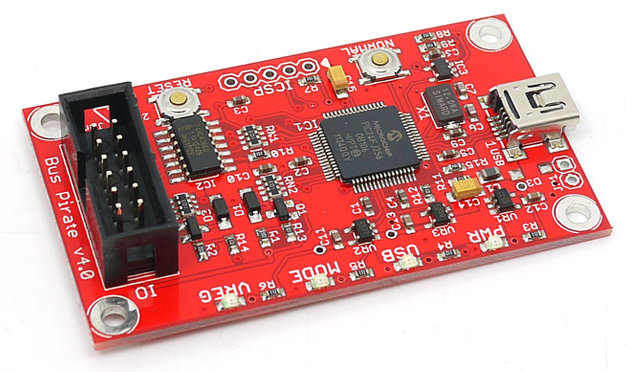
\includegraphics[width=0.5\textwidth] {img/buspirate.jpg}
	\caption{\label{fig:buspirate}Bus Pirate v.4 (picture by \textit{Seeed Studio})}
\end{figure}

%http://dangerousprototypes.com/blog/about/

% Dangerous Prototypes and manufactured by Seeed Studio\todo{link}
Bus Pirate, a project by Ian Lesnet, is a USB-attached device providing access to hardware interfaces like \gls{SPI}, \gls{I2C}, \gls{USART} and 1-Wire, as well as frequency measurement and direct pin access. The board aims to make it easy for users to familiarize themselves with new chips and modules; it also provides a range of programming interfaces for flashing microcontroller firmwares and memories. It communicates with the \gls{PC} using a FTDI USB-serial bridge.

Bus Pirate is open source and is, in its scope, similar to GEX. It can be scripted and controlled from the PC, connects to USB and provides a wide selection of hardware interfaces.

The board is based on a PIC16 microcontroller running at 32\,MHz. Its \gls{ADC} only has a resolution of 10 bits (1024 levels). There is no \gls{DAC} available on the chip, which makes applications that require a varied output voltage more difficult to implement. Another limitation of the board is its low number of \gls{GPIO} pins, which may be insufficient for certain applications. The Bus Pirate is available for purchase at around 30\,USD, a price comparable to some Raspberry Pi models.

\section{Professional DAQ Modules}

Various professional tools that would fulfill our needs exist on the market, but their high price makes them inaccessible for users with a limited budget, such as hobbyists or students who would like to keep such a device for personal use. An example is the National Instruments \IIC/SPI Interface Device which also includes several \gls{GPIO} lines, their USB DAQ module, or some of the Total Phase \IIC/SPI gadgets (figure \ref{fig:profidaq}). 

The performance GEX can provide may not always match that of those professional tools, but in many cases it'll be a sufficient substitute at a fraction of the cost.

\begin{figure}[h]
	\centering
	\begin{subfigure}{.5\textwidth}
		\centering
		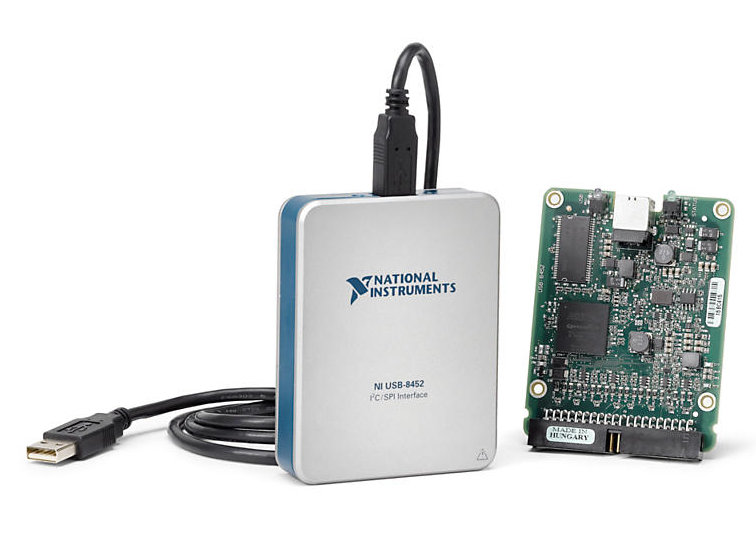
\includegraphics[width=.95\linewidth]{img/ni-i2c-device.jpg}
		\caption{NI \IIC/SPI Interface Device}
	\end{subfigure}%
	\begin{subfigure}{.5\textwidth}
		\centering
		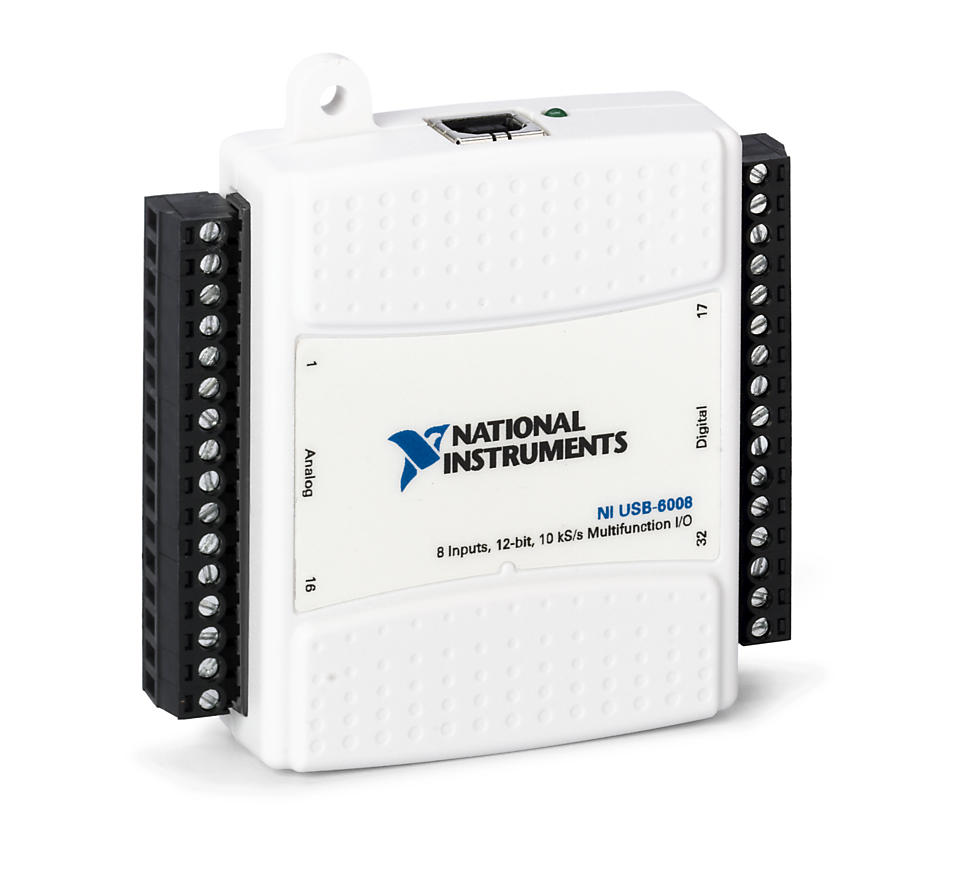
\includegraphics[width=.95\linewidth]{img/nidaq.jpg}
		\caption{NI USB DAQ module}
	\end{subfigure}
	\begin{subfigure}{.5\textwidth}
		\centering
		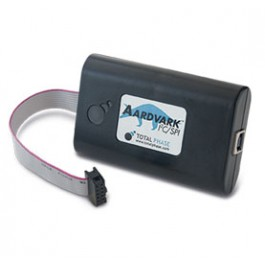
\includegraphics[width=.95\linewidth]{img/total-phase-spi-i2c.jpg}
		\caption{Total Phase SPI/\IIC Host "Aardwark"}
	\end{subfigure}
	\caption[Professional tools that GEX can replace]{\label{fig:profidaq}An example of professional tools that GEX could replace in less demanding scenarios \textit{(pictures from National Instruments and Total Phase marketing materials)}}
\end{figure}

%http://www.ni.com/en-gb/shop/select/i2c-spi-interface-device}

\iffalse
\section{The Firmata Protocol}

\todo[inline]{links}

Firmata is a communication protocol based on MIDI (\textit{Musical Instrument Digital Interface}) for passing data to and from embedded microcontrollers. MIDI is mainly used for attaching electronic musical instruments, such as synthesizers, keyboards, mixers etc., to each other or to a PC. Firmata was designed for Arduino as a high level abstraction for its connection to the PC, typically using a FTDI chip or equivalent.

Implementing Firmata in the GEX firmware would make it possible to use existing Firmata libraries on the PC side. However, the protocol is limited by the encompassing MIDI format and isn't very flexible. 
\fi

